\chapter{Analyse van het probleem}
\label{analyse}
Door zo veel mogelijk afhankelijkheden uit het configuratiemodel te halen kan een grote \todo{specifi\"eren hoeveel groter} tijdswinst behaalt worden tijdens het uitrollen van dat model.
Als de CMS beschikt over alle bestaande afhankelijkheden kan ze namelijk in \'e\'en keer het volledige model correct uitrollen.
Het doel is dus om niet alleen de afhankelijkheden te gebruiken die expliciet vermeld staan maar ook heuristieken te gebruiken om impliciete afhankelijkheden af te leiden.

Deze heuristieken worden toegepast eens het model volledig opgesteld en voordat het uitrollen begint.
Zo beschikken ze over alle nodige informatie en kan nog extra informatie toegevoegd worden aan het model.
Deze orde waarin deze heuristieken opgeroepen worden kan vastgelegd worden. Dit komt handig van pas bij het verwerken van relaties in het model, zie sectie \ref{relaties} en \ref{hoog_niveau_relaties}.

\section{Afhankelijkheden tussen bestanden en mappen}
\label{bestanden_en_mappen}
Tussen bestanden en mappen bestaat er zonder twijfel een sterke afhankelijkheid: een bestand kan helemaal niet bestaan zonder een map.
Visueel is dit voorgesteld in figuur \ref{fig:file_dir_dep}.
De eerste heuristiek die werd ontwikkeld voor IMP is er een die voor elk bestand de bijhorende map opzoekt in het model en een afhankelijkheid toevoegd als deze gevonden wordt.
Het algoritme dat hiervoor gebruikt wordt ziet eruit als volgt (pseudocode):

\begin{lstlisting}
foreach file in resources:
    foreach dir in resources:
        if get_directory(file.path) == dir.path:
            file.requires.append(dir)
\end{lstlisting}

Als de map niet vermeld wordt in het model wordt deze ook niet toegevoegd omdat dit ongewenste gevolgen kan hebben. \todo{Welke?}

\subsection{Resultaten}
\label{bestanden_en_mappen_res}
Om het effect van deze heuristiek te meten werden verschillende deployment runs gestart met en zonder gebruik van het algoritme.
Het resultaat van deze testen is te vinden in figuur \ref{fig:file_dir_times}.
Elk datapunt is het gemiddelde van 30 runs, uitgevoerd op een virtuele machine met 2 cores van 2 Ghz en 2 GB RAM ter beschikking.

\begin{figure}
    \label{fig:file_dir_times}
    \begin{center}
    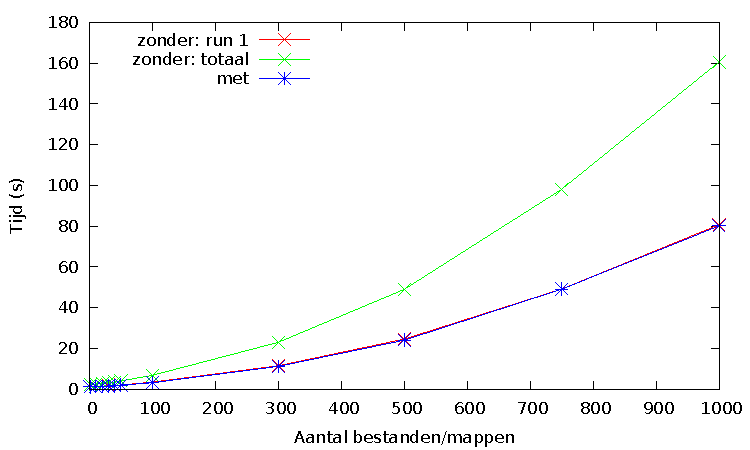
\includegraphics[width=0.8\textwidth]{images/file_dir_times.pdf}
    \caption{Testresultaten bij het uitrollen van een stijgend aantal bestanden en mappen, met en zonder gebruik van de heuristiek}
    \end{center}
\end{figure}

Hierop zien we duidelijk dat de heuristiek een sterke tijdswinst oplevert.
Het geoptimaliseerde uitrolproces heeft een quasi constante uitroltijd terwijl het standaardproces O(n) tijd nodig heeft.
Als geen afhankelijkheden worden toegevoegd is het aantal fouten tijdens het uitrollen namelijk evenredig met het aantal bestanden in het model.
Elk bestand heeft een kans van 50\% om uitgerold te worden v\'o\'or zijn map.
De stijgende lijn wordt dus verklaard door het stijgend aantal foutmeldingen.

Sowieso zijn er altijd maar maximaal twee deployment runs nodig als geen heuristiek gebruikt wordt aangezien mappen altijd kunnen gecre\"eerd worden.

\section{Afhankelijkheden tussen services, packages en configuratiebestanden}
\label{services_packages_en_configuratiebestanden}
Net zoals tussen bestanden en mappen is er een sterke afhankelijkheid tussen packages, services en hun eventuele configuratiebestanden:
een service kan niet gestart worden als zijn package niet ge\"installeerd is en zal niet correct werken zonder een aangepast configuratiebestand.
Een grafische voorstelling hiervan is te vinden op figuur \ref{service_package_dep}.

\begin{figure}
    \label{fig:service_package_dep}
    \begin{center}
    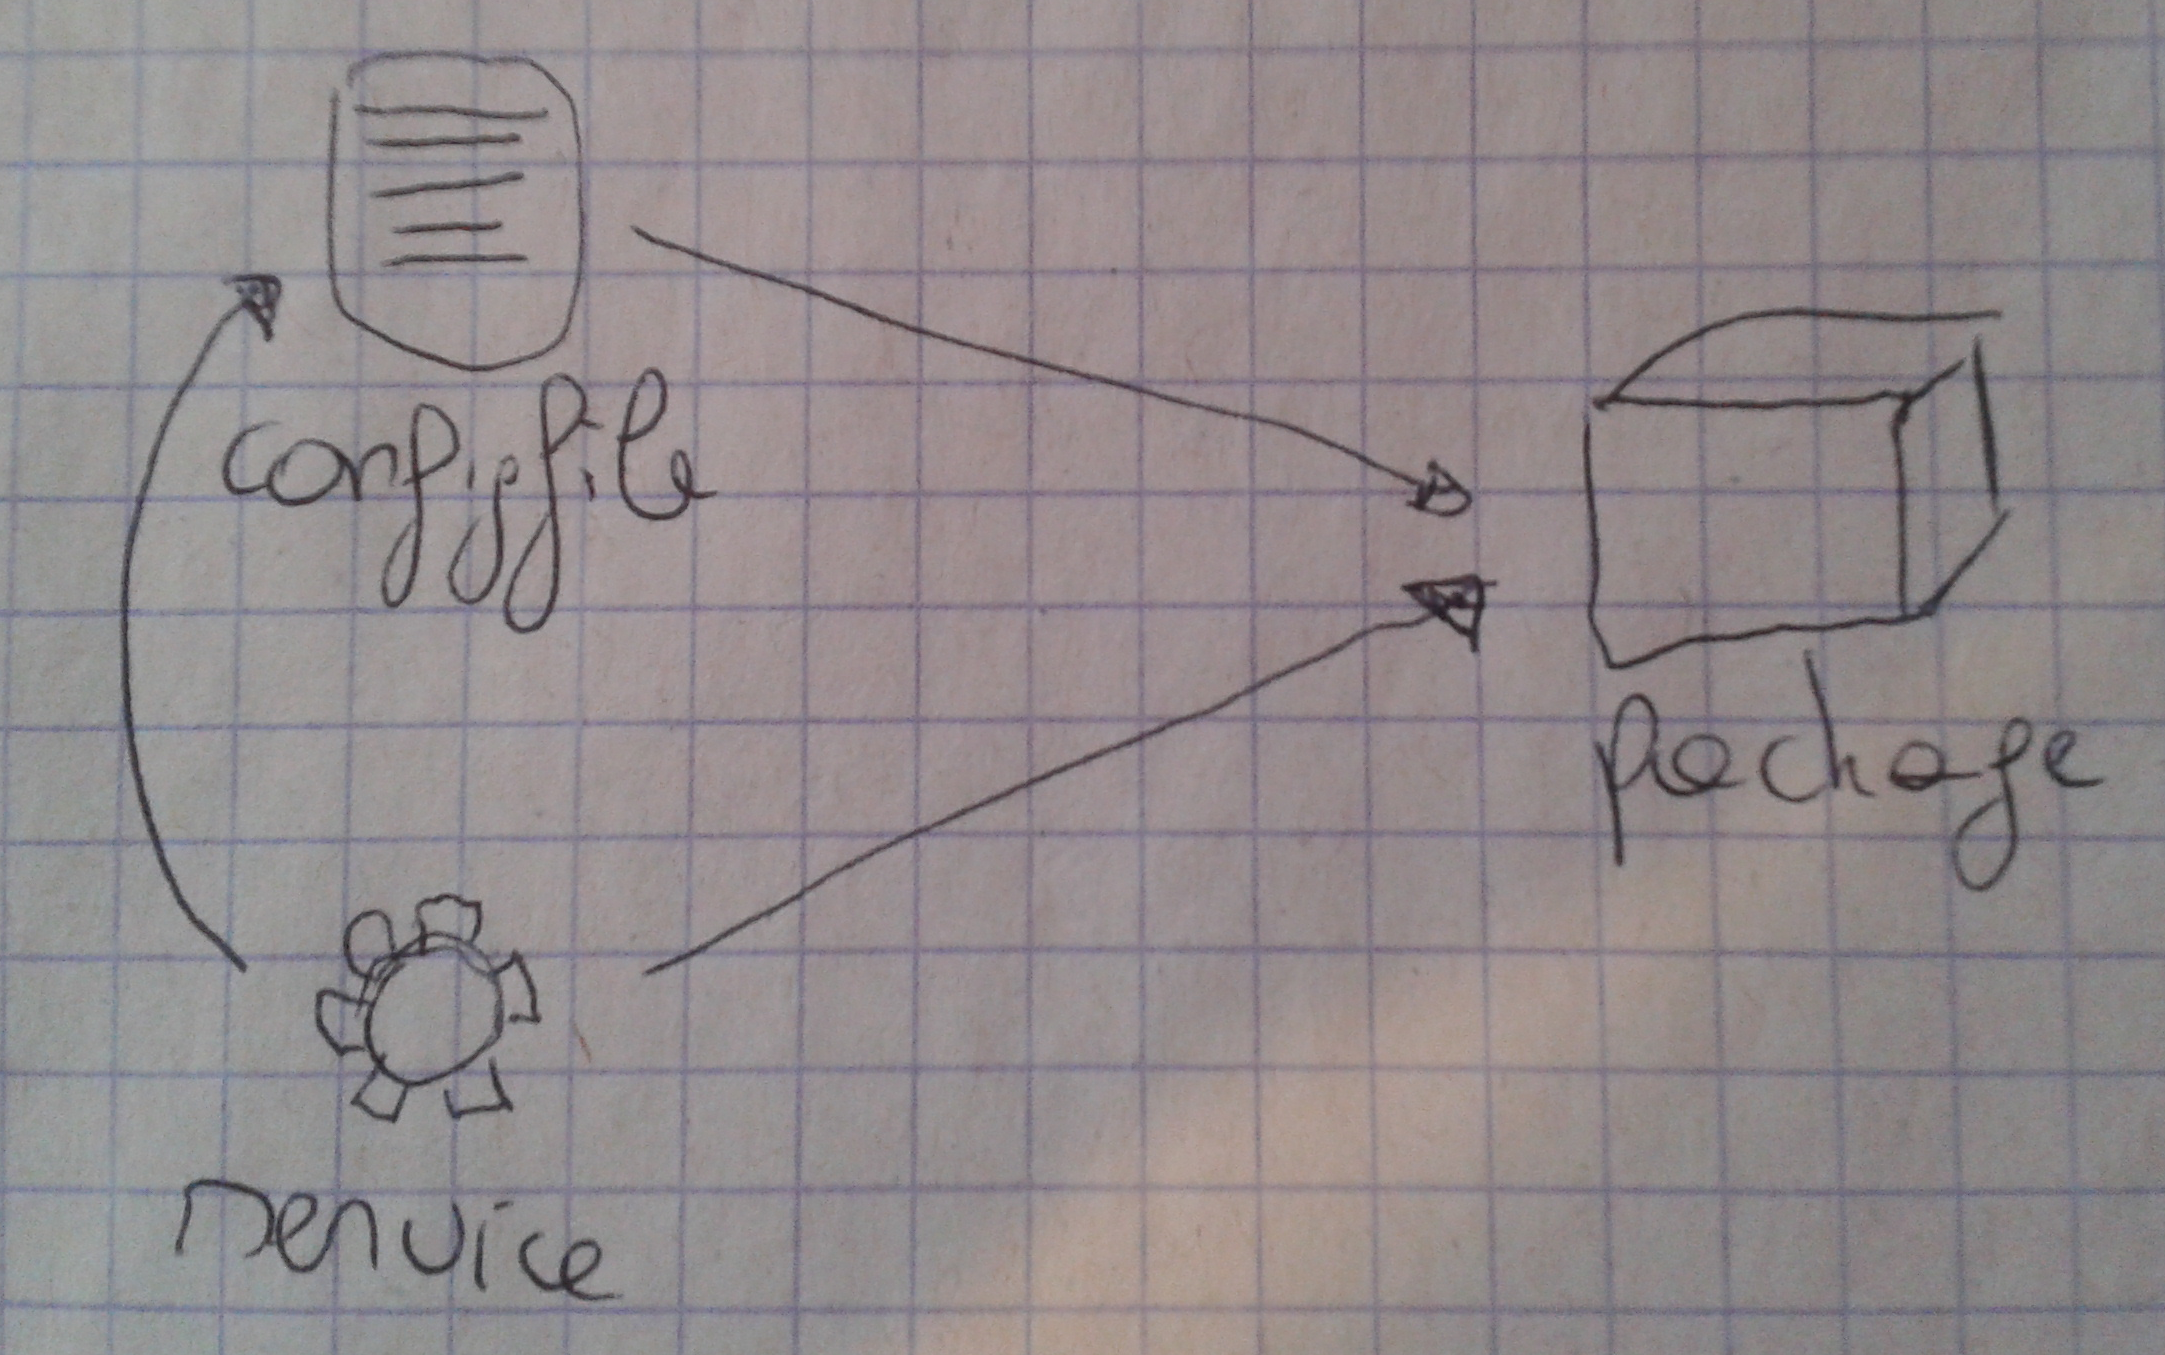
\includegraphics[width=0.6\textwidth]{images/service_package_dep.png}
    \caption{Grafische voorstelling van de afhankelijkheden die voorkomen tussen packages, services en configuratiebestanden}
    \end{center}
\end{figure}

De meest simplistische aanpak om de correcte afhankelijkheden te introduceren is alle services afhankelijk maken van alle packages en files en alle files afhankelijk van de packages.
De configuratiebestanden mogen pas geplaatst worden nadat de packages ge\"installeerd zijn omdat anders het aangepast configuratiebestand overschreven wordt.
Dit introduceert uiteraard veel afhankelijkheden die niet overeenstemmen met de werkelijkheid maar ze maken daardoor het resultaat van het uitrolproces niet fout.
Een algoritme in pseudocode ziet er uit als volgt:
\begin{lstlisting}
foreach service in resources:
    foreach file in resources:
        service.requires.append(file)
    foreach package in resources:
        service.requires.append(package)
foreach file in resources:
		foreach package in resources:
				file.requires.append(package)
\end{lstlisting}

De volgende aanpak gebruikt wat meer info uit het model en resulteert in minder overbodige afhankelijkheden.
In de modelcode worden bestanden, packages en services die bij elkaar horen meestal binnen eenzelfde implementatie gespecifi\"eerd.
Een voorbeeld is de implementatie van een MySQL server:
\begin{lstlisting}
implementation mysql:
    pkg = std::Package(host= host, name= "mysql-server", state= "installed")
    svc = std::Service(host= host, name= "mysqld", state= "running", onboot= true)

    config= std::ConfigFile(host= host, path= "/etc/my.cnf", content= template("mysql/my.cnf.tmpl"), requires= pkg, reload= true)
    conf_dir= std::Directory(host= host, path= "/etc/mysql.conf.d", owner= "root", group= "root", mode= 755)

    dblist= std::ConfigFile(host= host, path= "/etc/sysconfig/mysql", reload= true, content= template("mysql/databases.tmpl"))
end
\end{lstlisting}

Bij het verwerken van het model tijdens het uitrolproces bevinden al deze resources zich binnen dezelfde scope.
De heuristiek bestaat er uiteindelijk uit verzamelingen van packages en services te vinden die binnen \'e\'enzelfde scope gedefini\"eerd zijn en de correcte afhankelijkheden op te stellen tussen enkel die resources.
Deze verzamlingen worden "service stacks"  genoemd.
De aanwezigheid van files is optioneel: sommige servicen moeten niet verder geconfigureerd worden.
Algoritmisch ziet de code hiervoor  er uit als volgt (pseudocode):

\begin{lstlisting}
srv_stacks = []
for resource in resources:
    same_scope = [res in resources where res.scope == resources.scope]
    if same_scope.contains(services) and same_scope.contains(packages):
        srv_stacks.append(same_scope)

foreach stack in srv_stacks:
    foreach service in stack:
        foreach file in stack:
            service.requires.append(file)
        foreach package in stack:
            service.requires.append(package)
\end{lstlisting}


\section{Afhankelijkheden door relaties}
\label{relaties}
IMP laat toe in het model relaties tussen concepten te specifi\"eren.
Een voorbeeldrelatie is de volgende:
\begin{lstlisting}
BaseClient clients [0:] -- [0:] BaseServer servers
\end{lstlisting}
Deze betekent dat een BaseClient nul of meerdere BaseServers nodig heeft, en omgekeerd.
Een ander voorbeeld is 
\begin{lstlisting}
Host host [1] -- [0:] File files
\end{lstlisting}
Deze betekent dat op een Host nul of meerdere files kunnen staan, maar dat elke File \'e\'en Host moet hebben.
Hieruit kunnen we afleiden dat een File niet kan bestaan zonder een host en het dus nodig is dat eerst de Host moet bestaan en opgestart zijn voordat geprobeerd wordt de File te cree\"eren.

Algemeen kan men dus besluiten dat elke relatie waar de ene kant een multipliciteit van [0] of [0:] heeft en de andere kant multipliciteit [1] of [1:] de eerste entiteit afhankelijk is van de tweede.
De code voor deze heuristiek ziet er uit als volgt:
\begin{lstlisting}
for lib in model.get_scopes():
    for concept in lib.variables():
        if concept.hasattr(relation)
            if concept.relation.low == 0 and concept.relation.end == 1:
                concept.relation.depends = True
\end{lstlisting}

\section{Afhankelijkheden tussen hoog-niveau concepten}
\label{hoog_niveau_relaties}
IMP laat niet alleen toe om afhankelijkheden tussen enkelvoudige concepten zoals bestanden, services,\ldots te specifi\"eren maar ook tussen samengestelde concepten zoals webservers, databaseservers,\ldots
Deze betekenen dat de ene kant niet zijn volledige functionaliteit kan aanbieden zonder de aanwezigheid van de andere kant.
Aangezien functionaliteit meestal aangeboden wordt door services stelt deze heuristiek enkel afhankelijkheden op tussen services die gespecifi\"eerd zijn binnen elk concept.

IMP laat toe om verschillende libraries te gebruiken (en zelf te defini\"eren) met daarin voorgedefinieerde concepten. 
Het algoritme begint met het doorzoeken van deze libraries naar concepten die services bevatten.
Dan kijkt het of dat concept afhankelijk is van een ander concept.
Als dit het geval is wordt gekeken of dat ander concept ook services bevat.
Zo ja stelt het algoritme de nodige afhankelijkheden op.

In pseudocode ziet dit er uit als volgt:

\begin{lstlisting}
for lib in model.get_scopes():
    for concept in lib.variables():
        concept_services = get_services(concept)
        if concept_services is not None:
            for relation in concept.get_attributes():
                if relation.depends: #afhankelijke relatie
                    for instance in concept.values: #Voor elke instantie v/h concept
                        req_concepts = relation.end
                        req_resources = []
                        for req_concept in req_concepts:
                                for srv in get_services(req_concept):
                                    req_resources.append(srv)
                        if req_resources is not None: 
                            for service in concept_services:
                                for req_res in req_resources:
                                    service.requires.add(req_res)
\end{lstlisting}

Het is belangrijk dat deze heuristiek wordt opgeroepen na deze van sectie \ref{relaties}, daar worden namelijk extra afhankelijke relaties opgesteld die hier kunnen gebruikt worden.
\section{Besluit van dit hoofdstuk}
